\chapter{Firmware Modules $\&$ Settings}
\label{chap:firmware}

\section{SVN Structure}

The SVN structure used for the \gls{deap3} firmware depicted in Fig. \ref{Fig:firmHier} has two main logical parts, the physics payload (red) and the \gls{fmc} drivers/software (blue) combined as SVN externals to the top project (green). 
The modules pertaining to the function of the trigger is considered the physics payload and is made up of  edevel00261 (Section \ref{sec:261}), edevel00260 (see Section \ref{sec:260}), and parts of edevel00270 (Section \ref{sec:270}). 
The rest of the drivers and control code is apart from the trigger itself and is beyond the scope of this manual. 
For more specifics on the driver firmware look at the repository\footnote{\url{https://edev.triumf.ca/project/deap/edevel00013}}, or contact Yair Linn\footnote{yairlinn@triumf.ca} or Daryl Bishop\footnote{daryl@triumf.ca}. The firmware pertaining to the trigger and general operation of the \gls{dtm} follow.

\begin{landscape}
	\vspace*{\fill}
	\begin{figure}[ht]
	\centering
	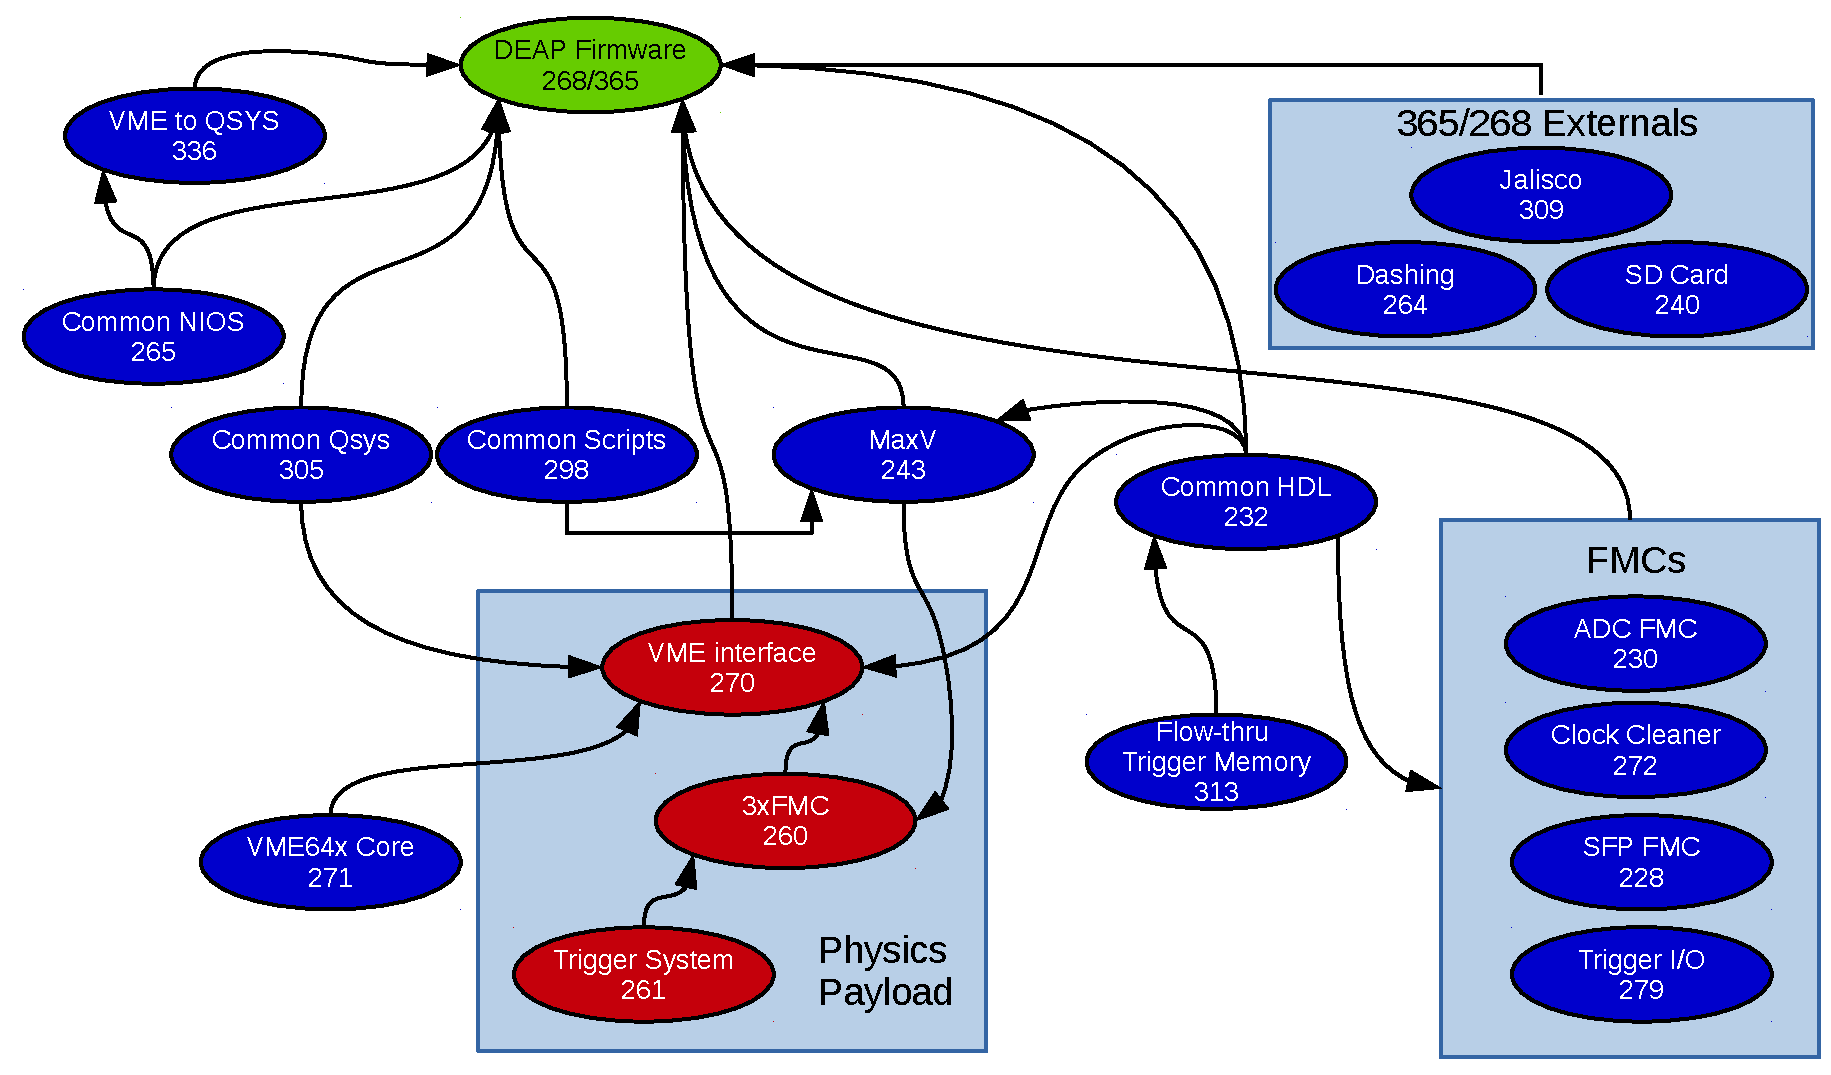
\includegraphics[width = .73\paperheight]{firmwareHier}
	\caption{Flow chart of the firmware SVN structure. The top project is either edevel00268 or edevel00365 with the various other projects connected as externals. The modules in blue are maintained by the TRIUMF EDEV department whereas the modules in red (the physics payload) is maintained by \gls{deap3}. The externals for 268 and 365 are identical as shown.}
	\label{Fig:firmHier}
	\end{figure}
	\vspace*{\fill}
\end{landscape}


\section{Trigger System (edevel00261)}
\label{sec:261}
\begin{description}
\item[SVN Location:] https://edev.triumf.ca/svn/edevel00261
\item[Last Installed Tag:] \tagTwoSixOne %this is defined in triggerManual.tex at the start of the document
\item[Externals:] None
\item[Summary:] The trigger system code contains all of the trigger modules and submodules which are called into the \gls{vme} interface (Section \ref{sec:270}). All the trigger modules described in Chapter \ref{chap:triggers} are located in tsb/ip/rtl/source. The other trigger system modules are introduced below.
\end{description}
	

	
	\subsection{Baseline Compensation}
	\label{sec:baseline}
	\begin{description}
	\item[Module Name:] trigger\_baseline
	\item[SVN Location:] \url{https://edev.triumf.ca/svn/edevel00261/trigger\_baseline.v}
	\item[Modules used in:] ts\_adc $\&$ min bias, deap\_vme\_interface\_wrapper.v 
	\end{description}
	
	
	\begin{figure}[ht]
	\centering
	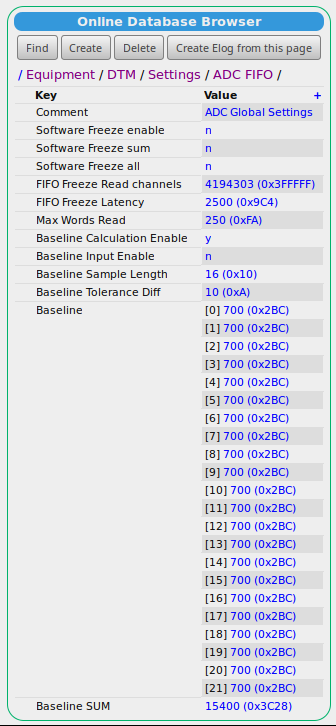
\includegraphics[height = .8\paperheight]{adcFIFO}
	\caption{Online data base settings for the ADC FIFO and baselines.}
	\label{Fig:adcFIFO}
	\end{figure}
	
	
	The ADC baseline compensation module is a module designed for the ADC trigger (Section \ref{sec:adcTrig}) source to allow the calculation of \gls{fprompt}. The minimum bias trigger (Section \ref{Fig:minBiasTrigger}) is also configured for it, but there is little motivation to use it as absolute ADC threshold values are equivalently useful.
	
	The baseline calculation is preformed with an averaging function that sums ADC data (each \gls{asum} channel has its own compensation module) for 2$^n$ bins (the value of n is set in the \gls{odb}, a common value is 16 bins, i.e. n = 4). The sum is then right shifted by n bits giving the average value of the 2$^n$ bins.
	A default value is set in the \gls{odb} and is used as the starting baseline. This value can remain static, an external baseline can be inputed, or a dynamic calculation can be enabled.
	
		\subsubsection{Baseline Calculation}
		
		If placed in baseline calculation mode as is typical to allow for some drift as is expected from the PMTs, the baseline will dynamically calculated and adjusted. Every 2$^n$ clocks the baseline is re-averaged in the manner described above. This new value is compared to the previously set baseline and the difference is recorded. This repeats with the difference between the set and re-averaged baselines being summed each time. If the difference exceeds the tolerance set in the \gls{odb} then the set baseline is incremented by one in the direction of the trend. If the difference exceeds the tolerance the set baseline is incremented by one as the baseline is tending low. If the difference is less than the negative tolerance, the set baseline is decremented by one as the baseline is tending high.
		
		The algorithm starts to run after the DTM is booted, so before the start of the run. However, it is reset at each start of run by the frontend. The baselines of all channels are not currently\footnote{July, 2016} saved into the data structure, however the long term stability can be seen on the front end.
		
		Although previously the \gls{ass} baseline was calculated as the sum of the \gls{asum} baselines (as stated in the twiki\footnote{\url{https://www.snolab.ca/deap/private/TWiki/bin/view/Main/DTMBaseline}} location), this baseline is calculated separately from the sum of the signals.
		
		\NOTE{The change of the \gls{ass} baseline calculation is to remove the offset caused by truncation, with 22 channels the truncation error would average 11 ADC off.}

		\subsubsection{Baseline Stability}
		\begin{description}
		\item[\gls{odb} Baseline Plot: ]\url{https://deapdaqgw.snolab.ca/HS/Baseline/}	
		\end{description}
		The baseline values are not currently\footnote{July, 2016} readout into the RAT data structure, however the stability can be monitered online at the location given above. Each of the \gls{asum} baselines (Fig. \ref{Fig:baselineStabilityAsum1}  and Fig. \ref{Fig:baselineStabilityAsum2} ) are monitered as well as the \gls{ass} (Fig. \ref{Fig:baselineStability}). 
		
		\NOTE{The three day monitering is shown in Fig. \ref{Fig:baselineStabilityAsum1} - \ref{Fig:baselineStability} but this plot goes from 10 min to 7 days and of course can be configured to other times.}
		
		\begin{figure}[ht]
		\centering
		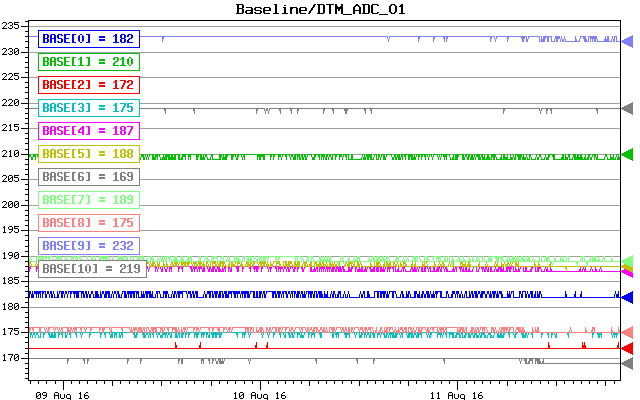
\includegraphics[width = .8\textwidth]{DTM_ADC_01}
		\caption{Long time plot of the first 11\gls{asum} baselines over a 3 day period. Each baseline is continuously calculated and allowed to change.}
		\label{Fig:baselineStabilityAsum1}
		\end{figure}		
		
		\begin{figure}[ht]
		\centering
		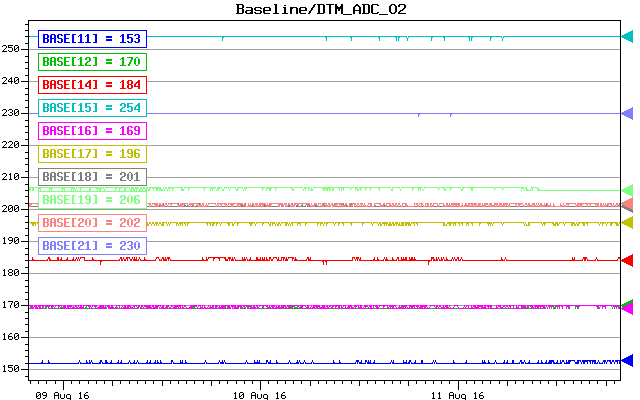
\includegraphics[width = .8\textwidth]{DTM_ADC_02}
		\caption{Long time plot of \gls{asum}s 11-21 baselines over a 3 day period. Each baseline is continuously calculated and allowed to change.}
		\label{Fig:baselineStabilityAsum2}
		\end{figure}
						
		\begin{figure}[ht]
		\centering
		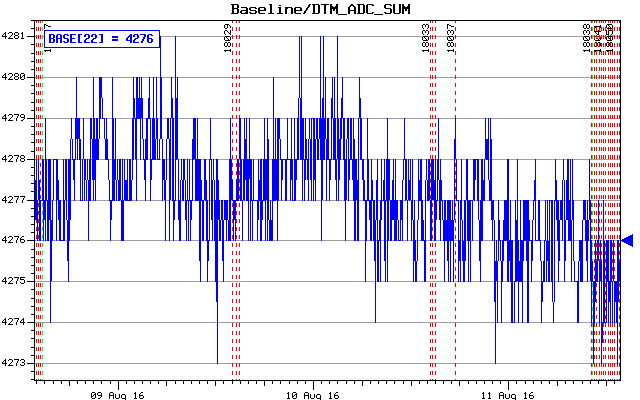
\includegraphics[width = .8\textwidth]{baselineStability}
		\caption{Long time plot of the \gls{ass} baseline over a 3 day period. The baseline is continuously calculated and allowed to change.}
		\label{Fig:baselineStability}
		\end{figure}		
						
	
	\clearpage
	\subsection{Self Sum Module}
	\label{sec:selfSum}
	\begin{description}
	\item[Module Name:] trigger\_self\_sum\_adc
	\item[SVN Location:] tsb/ip/rtl/trigger\_self\_sum\_adc.v
	\item[Modules used in:] TriggerSourceADC
	\item[Summary:] Returns the integrated charge within a defined short and long time window of the baseline subtracted (see above) \gls{ass} continuously. Both integrations start at the same time, so the short time window result is held in a FIFO with respect to the end of the long time window so that both results are present at the same time. The maximum values for windows are 50 \gls{dtm} clocks for the short window (TICKS\_SHORT = 50) and 500 \gls{dtm} clocks for the long window (TICKS\_LONG = 500). At 22.14 ns these max times are 1107 ns and 11070 ns respectively. %Clock domain change from ADC clock (45.161290 MHz) to DAQ clock (62.5 MHz) is provided using FIFOs.
	\end{description}
	
	
	\subsection{Trigger Self Decision Module}
	\label{sec:trigSelfDecision}
	\begin{description}
	\item[Module Name:] TriggerSelfDecision
	\item[SVN Location:]  tsb/ip/rtl/trigger\_self\_decision.v
	\item[Modules used in:] TriggerSourceADC
	\item[Summary:] The self decision module uses the short and long integrated \gls{ass} windows passed by the trigger\_self\_sum\_adc module (See above). As described in Section \ref{sec:adcTrig} and shown in Fig. \ref{Fig:triggerRegions} there are 4 energy regions: very low (or noise), low, high, and very high with the low and high regions being separated by their \gls{fprompt}. Energy selection is done by simply comparing the set threshold to the short energy from the self sum module. The energy is sorted into very high, then high, then low. The \gls{fprompt} selection is done by left shifting the short charge by eight bits and comparing that value to the \gls{fprompt}s for each region (as set in the \gls{odb} as a value [1-256]) multiplied by the long window charge. The highest energy followed by highest \gls{fprompt} is set first.
	\end{description}
	
	\subsection{Trigger Top Module}
	\label{sec:trigTop}
	\begin{description}
	\item[Module Name:] DEAPTriggerTop
	\item[SVN Location:]  tsb/ip/rtl/trigger\_top.v
	\item[Modules used in:] vme wrapper
	\item[Summary: ]Trigger top level module. Calls TriggerNIMIO, TriggerEventArbiterWithFIFO, and TriggerPrescalerWithFIFO. This module looks after what happens after one of the enabled triggers puts out a signal, contains the NIM output control. Runs on the 62.5 MHz \gls{daq} clock. Prescales events and takes care of collisions of events in TriggerEventArbiterWithFIFO. The event data written to the arbiter \gls{fifo} is passed to VME\_MAPPED\_REGFILE\_STATUS which is then read out by \gls{midas}. 
	
	\NOTE{It was being talked about adding a shutdown if events come too quickly, that could either be done here or in TriggerEventArbiterWithFIFO.}	
	\end{description}	
	
		\subsubsection{Trigger Event Arbiter With FIFO}
		\label{sec:triggerEventArbiterWithFIFO}
		\begin{description}
		\item[Module Name:] TriggerEventArbiterWithFIFO
		\item[SVN Location:]  tsb/ip/rtl/trigger\_event.v
		\item[Modules used in:] DEAPTriggerTop
		\item[Summary:] Deals with what event from the prescalers gets sent through and written to a \gls{fifo}. Reads through events in prescalers by Round Robin Arbitration (One clock cycle per prescaler). Checks all the other prescalers if an event with the same timestamp is available if they are then they are merged if not, but another event with an earlier timestamp is available, buffer the first event and go to the earlier one. If no other event with the same or earlier timestamp is available then the event is written to the \gls{fifo}. This method ensures that although there are several different triggers, the ones written out to \gls{midas} are all is sequential order.
		
		\NOTE{It was being talked about adding a shutdown if events come too quickly, that could either be done here or in DEAPTriggerTop.}
		\end{description}
	
		\subsubsection{Trigger Prescaler With FIFO}
		\label{sec:trigPrescaleFifo}
		\begin{description}
		\item[Module Name:] TriggerPrescalerWithFIFO
		\item[SVN Location:]  tsb/ip/rtl/trigger\_prescaler\_fifo.v
		\item[Modules used in:] DEAPTriggerTop
		\item[Summary:] Calls TriggerPrescaler and writes a \gls{fifo} with all of the trigger information for readout by TriggerEventArbiterWithFIFO. The trigger information is saved in a \gls{fifo} until called. Each trigger type has its own \gls{fifo} of nominally 16 words deep. If the module receives a trigger it will write the trigger information to the \gls{fifo} and the sequential events will be readout by the arbiter.
		\end{description}
		
		
		\subsubsection{Trigger Prescaler}
		\label{sec:trigPrescaler}
		\begin{description}
		\item[Module Name:] TriggerPrescaler
		\item[SVN Location:]  tsb/ip/rtl/trigger\_prescaler.v
		\item[Modules used in:] TriggerPrescalerWithFIFO
		\item[Summary:] Counts the number of triggers that come in and output one once the set prescale amount is met. Syncs the various event builder data so that the output of the trigger is valid with the values of the short/long ADC integrated charge or the number of coincidence channels from the Min. bias trigger. 
		\end{description}
	

		\subsubsection{Trigger NIM I/O}
		\label{sec:triggerNIMIO}
		\begin{description}
		\item[Module Name:] TriggerNIMIO
		\item[SVN Location:]  tsb/ip/rtl/trigger\_nim\_io.v
		\item[Modules used in:] DEAPTriggerTop
		\item[Summary:] Trigger output module. This module receives a trigger signal in for one of its 8 output channels. The module checks to see if the suppression time since the last output on that channel has been exceeded yet, if it has and the busy signal is false the trigger count for that channel is incriminated and a trigger signal is sent out of the designated output. If the busy input on the NIM I/O \gls{fmc} is high then no trigger output can occur\footnote{For more on the busy signals see the twiki: \url{https://www.snolab.ca/deap/private/TWiki/bin/view/Main/InfoBusy}}.
		\end{description}
	

	
\section{3xFMC (edevel00260)} 
\label{sec:260}
\begin{description}
\item[SVN Location:] https://edev.triumf.ca/svn/edevel00260
\item[Last Installed Tag:] \tagTwoSixZero %this is defi/tsbs/deap_vme_and_daq/tsbs/trigger_and_daq/ned in triggerManual.tex at the start of the document
\item[Externals:] MaxV (edevel00243), TriggerSystem (edevel00261) 
\item[Summary:] Contains the NIOS core for the exponential trigger, the software which generates the exponential random number and the global parameters used in the trigger system (parameters.v).
\end{description}
\NOTE{Contains the global parameters for the trigger system in parameters.v}

\section{DEAP VME Interface (edevel00270)} 
\label{sec:270}
\begin{description}
\item[SVN Location:] https://edev.triumf.ca/svn/edevel00270
\item[Last Installed Tag:] \tagTwoSevenZero %this is defi/tsbs/deap_vme_and_daq/tsbs/trigger_and_daq/ned in triggerManual.tex at the start of the document
\item[Externals:] Common QSYS (edevel00305), Common HDL (edevel00232), VME64x Core (edevel00271), 3xFMC (edevel00260)
\item[Summary:] The VME Interface is the top SVN project of the physics payload as shown in Fig. \ref{Fig:firmHier}. Although not containing any of the actual \gls{fmc} drivers themselves, this project encapsulates all of the data taking and processing as well as all of the triggers and event selection.
\end{description}

	\subsection{VME Interface Wrapper} 
	\label{sec:vmeWrapper}
	\begin{description}
	\item[Module Name:] deap\_vme\_interface\_wrapper
	\item[SVN Location:]  tsb/ip/rtl/deap\_vme\_interface\_wrapper.v
	\item[Modules used in:] VME\_3xFMC\_Carrier (edevel00365 or edevel00268 in tsb/ip/rtl/VME\_3xFMC\_Carrier.v)
	\item[Summary: ]This is the top level verilog file of this subproject. Instantiates the DEAP trigger sources, ADC \gls{vme} \gls{fifo}s, \gls{deap} trigger top module, exponential trigger NIOS, \gls{vme} registers and their assignments. Anything related to the ADC Waveform FIFOs is to be done in this file. This module contains all of the physics level firmware.
	\end{description}

	

\section{DEAP Firmware Development Quartus 13.0sp1 (edevel00268)} 
\label{sec:268}
\begin{description}
\item[SVN Location:] https://edev.triumf.ca/svn/edevel00268
\item[Last Installed Tag:] \tagTwoSixEight %this is defined in triggerManual.tex at the start of the document
\item[Externals:]  \gls{jalisco} (edevel00309), Dashing (edevel00264), SD Card (edevel00240), VME to QSYS (edevel00336), MaxV (edevel00243), Common NIOS (edevel00265), Common QSYS (edevel00305), Common Scripts (edevel00298), Common HDL (edevel00232), ADC FMC (edevel00230), Clock Cleaner (edevel00272), SFP FMC (edevel00228), Trigger I/O (edevel00279), VME Interface (edevel00270)
\item[Summary: ]Currently edevel00268 is the top SVN project for \gls{deap3}. Each of the preceding files and projects described above (excluding edevel00268) are included as externals. 268 uses the master clock distribution \gls{fmc} board (see Section \ref{sec:mClockBoard}) with daisy chain clocking. 268 has experienced issues operating on the 3xFMC Rev. A board and therefore is only used with the Rev. B board (See the Errata \ref{chap:errata}). See Section \ref{sec:dtmConfigs} for the applicable hardware configuration. The programming scripts for the FPGAs are located in tsb/ip/scripts\footnote{see Chapter \ref{chap:install} for programming} with the binary files to be loaded held in tsb/ip/exe.

\NOTE{It is crucial to make sure the correct \gls{fmc}s are connected, \textbf{do not} load 268 with the SFP and Mini-Sas board attached and \textbf{do not} load 365 with the Clock distribution \gls{fmc}.} 
\end{description}

	\subsection{VME 3xFMC Carrier} 
	\label{sec:VME_3xFMC_Carrier268}
	\begin{description}
	\item[Module Name:] VME\_3xFMC\_Carrier
	\item[SVN Location:]  tsb/ip/rtl/VME\_3xFMC\_Carrier.v
	\item[Modules used in:] N/A (Top Project Module)
	\item[Summary: ]This is the very top module of the \gls{deap3} firmware, and instantiates the deap\_vme\_interface\_wrapper module. This module is maintained exclusively by Yair Linn\footnote{yairlinn@triumf.ca}.
	\end{description}


\section{DEAP Firmware Quartus 14.1 (edevel00365)}
\label{sec:365}
\begin{description}
\item[SVN Location:] https://edev.triumf.ca/svn/edevel00365
\item[Last Installed Tag:] \tagThreeSixFive %this is defined in triggerManual.tex at the start of the document
\item[Externals:]  \gls{jalisco} (edevel00309), Dashing (edevel00264), SD Card (edevel00240), VME to QSYS (edevel00336), MaxV (edevel00243), Common NIOS (edevel00265), Common QSYS (edevel00305), Common Scripts (edevel00298), Common HDL (edevel00232), ADC FMC (edevel00230), Clock Cleaner (edevel00272), SFP FMC (edevel00228), Trigger I/O (edevel00279), VME Interface (edevel00270)
\item[Summary: ]Like edevel00268, edevel00365 is the top SVN project for \gls{deap3}, however the upgrade has not yet occurred\footnote{Upgrade date as yet unset (as of July 2016)}. Each of the preceding files and projects described above (excluding edevel00268) are included as externals. 365 uses the SFP and Mini-Sas \gls{fmc} board (see Section \ref{sec:SFPBoard}) adding FTP connectivity to the \gls{dtm} (see Chapter \ref{chap:install}). Additionally 365 has tighter timing constraints which has fixed the issues experienced with using 268 on the 3xFMC Rev. A board so may operate on either board (See the Errata \ref{chap:errata}). See Section \ref{sec:dtmConfigs} for the applicable hardware configuration. The programming scripts for the FPGAs are located in tsb/ip/scripts\footnote{see Chapter \ref{chap:install} for programming} with the binary files to be loaded held in tsb/ip/exe.

\NOTE{It is crucial to make sure the correct \gls{fmc}s are connected, \textbf{do not} load 268 with the STP and Mini-SAS board attached and \textbf{do not} load 365 with the clock distribution \gls{fmc}.} 

	\subsection{VME 3xFMC Carrier} 
	\label{sec:VME_3xFMC_Carrier365}
	\begin{description}
	\item[Module Name:] VME\_3xFMC\_Carrier
	\item[SVN Location:]  tsb/ip/rtl/VME\_3xFMC\_Carrier.v
	\item[Modules used in:] N/A (Top Project Module)
	\item[Summary: ] This is the same module as used in edevel00268 with several significant changes. This module is maintained exclusively by Yair Linn\footnote{yairlinn@triumf.ca}.
	\end{description}
	
\end{description}
